%======================================================================
% To compile this file you have to set the .tex file path:
% setenv TEXINPUTS .:${PWD}/../../../::
%
% Use latex or pdflatex to compile.
%
% Author: C.Leonidopoulos, E. Meschi (parts stolen from N. Amapane)
% $Date: 2006/12/18 23:35:00 $  $Revision: 1.9 $
%
%======================================================================
\documentclass[a4paper]{cmspaper}
\usepackage{lineno} % line numbering for draft
\usepackage{ifthen}

%======================================================================
% Check for PDFLaTeX/LaTeX 

\newif\ifpdf
\ifx\pdfoutput\undefined
\pdffalse 
\else
\pdfoutput=1 
\pdftrue
\fi

\ifpdf  % ============== we are running PDFLaTeX
\usepackage{color}
\usepackage[pdftex]{graphicx,graphics}
\usepackage{epsfig}
\usepackage{pdflscape}
\usepackage[bookmarksnumbered,bookmarksopen,bookmarksopenlevel=1,
              colorlinks,
              linkcolor=blue,                      
              citecolor=blue, 
              urlcolor=blue]{hyperref}                                 
\pdfinfo{
  /Title  (Design and Operation of the DQM Infrastructure)
  /Author (...)
  /Keywords (DQM, Online, DAQ, CMS)
  }

\DeclareGraphicsExtensions{.pdf}

\else   % ============== we are not running PDFLaTeX
\usepackage{epsfig}
\usepackage{lscape}

\special{!userdict begin /bop-hook{gsave 200 30 translate
         65 rotate /Times-Roman findfont 216 scalefont setfont
         0 0 moveto 0.93 setgray (DRAFT) show grestore} def end}

\DeclareGraphicsExtensions{.eps}

%fake pdflatex commands.
\newcommand{\pdfbookmark}[3][1]{}
\newcommand{\href}[2]{#2}

\fi

%==============================================================================


\newcommand {\ie}{\mbox{\sl i.e. }}     %i.e.
\newcommand {\eg}{\mbox{\sl e.g. }}     %e.g.


\begin{document}

%==============================================================================
% title page for few authors

\begin{titlepage}

% select one of the following and type in the proper number:
%   \cmsnote{2005/000}
  \cmsnote{2007/XYZ}
%  \conferencereport{2005/000}
   \date{\today}
\smallskip
\smallskip
 \rightline{\bf Version 1.0}


  \title{Design and Operation of the CMS Physics and Data Quality
Monitoring Infrastructure}

  \begin{Authlist}
    C.~Leonidopoulos, E.~Meschi, I.~Segoni and D.~Tsirigkas
       \Instfoot{cern}{CERN, Geneva, Switzerland}
    G.~Eulisse
       \Instfoot{nort}{Northeastern University, Somewhere-In-The-States, USA}
  \end{Authlist}

% if needed, use the following:
%\collaboration{Flying Saucers Investigation Group}
%\collaboration{CMS collaboration}

  \begin{abstract}
    \pdfbookmark[1]{Abstract}{Abstract}
  This note describes the architecture and implementation of
the CMS Physics and Data Quality Monitoring infrastructure. The DQM system 
underwent its first real-life test during the CMS Magnet Test and 
Cosmic Challenge (MTCC) in 2006, where a significant fraction of
the sub-detectors composing CMS where operated together and read-out using 
final front-end electronics and the general DAQ system. Experience 
of the use of the DQM during the MTCC is reported and perspectives 
for LHC-beam operation of CMS in 2007-2008 are discussed.
  \end{abstract} 

% if needed, use the following:
%\conference{Presented at {\it Physics Rumours}, Coconut Island, April 1, 2005}
%\submitted{Submitted to {\it Physics Rumours}}
%\note{Preliminary version}
  
\end{titlepage}

\setcounter{page}{2}%JPP
\linenumbers
%==========================================
\section{Introduction} \label{sec:introduction}
%\pdfbookmark[1]{Introduction}{Introduction}
%==========================================
%
The Physics and Data Quality Monitoring system (DQM) aims at
providing a homogeneous monitoring environment across various
applications related to data taking at CMS. Its infrastructure must be fairly
flexible and easily customizable so as to be usable by different
groups across the experiment. Applications that can
benefit from a unified approach to monitoring range from the high-level
trigger algorithms in the Filter Farm to local DAQ supervision by a subdetector group
up to
off-line reconstruction jobs carrying out ``production validation''.
The primary goal of the DQM system is however to guarantee the quality of physics data
collected by the general data acquisition.

The DQM infrastructure provides a generic interface
independent of the specific technology implementation
for the  creation and update of monitoring objects (e.g. histograms),
allowing direct insertion of monitoring statements in the reconstruction code.
Producers publish a list of available information
to be delivered to consumers upon connection. They accept subscription
requests for delivery of regular updates of a given piece of information.
The DQM infrastructure provides functionality to collect and organize information received
from a number of producers, and redirect it to consumers according to their
subscription requests. This interface can be accessed from standalone
programs, or can be used from within reconstruction applications and
modules. On the client side, tools are provided for evaluating the
consistency of received information to reference information retrieved from
a database, update these references, set thresholds, raise alarms, and
create error messages for use by the central error logging facility.
%
%
%==========================================
\section{Architecture} \label{sec:architecture}
%\pdfbookmark[1]{Architecture}{Architecture}
%==========================================
%
The DQM framework is designed to deal with sets of objects (``{monitoring
elements}'', or ME) from the creation in monitoring producers (``{sources}''),
to the organization and
redistribution, on a periodical basis, in the ``{collectors},'' to their final use
by {clients}. Sources are defined as
individual nodes that have either direct access to or can process and
produce information we are interested in. The creation and update of
MEs at the source can be the result of processing input event data
(event consumers) or input monitor elements (monitor consumers).

At the other end of this architecture are the monitoring information
consumers (``{clients}''). Clients are notified of available monitoring
information (``{monitorables}'') from all sources combined. They can
subscribe to and receive periodic updates of any desired subset of the
monitorables, in a classic implementation of the ``publish-subscribe'' service.
A hierarchical system of collector nodes is responsible for
the communication between sources and clients (e.g. subscription
requests) and the actual monitoring transfer. These nodes serve as
collectors for the sources and as monitoring servers for the clients.

In order to minimize the interference with the ``main'' application
running in the source process (e.g. analysis, calibration/alignment, trigger
algorithm, etc), DQM operations at the source are reduced to a
minimum. All CPU-intensive tasks (e.g.
comparison to reference monitoring element, display, database storage,
etc.) are to be carried out at the client's side.

The above design aims at
\begin{itemize}
\item{shielding the sources from connecting clients
that could slow down the main application or threaten the stability of
the source}
\item{facilitating the quick
transfer of the monitoring information from the sources to the collectors.}
\end{itemize}
To this end, sources are connected to only 1 collector each
(but a collector can connect to multiple sources). Clients do not have
direct access to the sources. All source-client communication is carried out
through the collector (or collectors).

In this design, the production of the monitoring information is clearly
separated from the collection and the processing. The collectors act as
the ``middle man'': they are responsible for advertising the monitorables
to different clients and serve monitoring requests.
The nature of the collection and processing of the monitoring
information is statistical by construction. In particular, the DQM
\begin{itemize}
\item{is meant to help the experts identify problems that occur (and are monitored)
\emph{over a period of time} and is not expected to be capable of spotting
punctual problems}
\item{does \emph{not} give
access to particular events}
\item{does \emph{not} guarantee that two clients
will receive identical monitoring information}
\end{itemize}
%
%
%==========================================
\subsection{Components and Data Flow}\label{sec:dataflow}
%\pdfbookmark[1]{DataFlow}{DataFlow}
%==========================================
%
\label{sec:req_general}
The DQM infrastructure supports various monitorable types.
1D-, 2D- and 3D-histograms,
1D- and 2D-profiles, scalars (integer and real numbers) and string messages
can be booked and filled/updated anywhere in the
context of reconstruction and analysis code.
The infrastructure takes
care of publishing, tracking updates, and transporting these updates to
subscriber processes. The
DQM infrastructure does \emph{not} provide support for publishing/transport of individual event
data. Distribution of data to ``event consumers'' is provided by a separate
system ({\it refer to section on EventServer/EventProxy} ).
Access to booking, filling and modifying MEs is provided via abstract
interfaces in every component. MEs are organized in
%UNIX-like
directory
structures with
virtually unlimited depth, from which monitor consumers can ``pick
and choose''.
In every component, it is possible at any point in time to create
root-tuples with ``snapshots''
of the monitoring structure for debugging and reference.

\subsubsection{Sources}
\label{sec:req_sources}

Data Quality Monitoring services available to the source not only keep track of updates to
existing monitor elements, they also enable dynamic modifications to the
monitoring structure. The list of available monitoring information
can be modified at run-time by booking or deleting MEs via the public
DQM service interface.
Updated information from an individual source is distributed to all
consumers (through the collector) by an update
task (MonitorDaemon) running periodically is a separate thread of the source
process.
The interval between 2 MonitorDaemon updates,
which defines a monitoring cycle, can be configured
for each individual source process.
A ``reset'' switch can be used to specify for each ME
whether monitoring contents
should be reset at the end of a cycle\footnote{This option should be
turned on for MEs that describe dynamic content (e.g. hit
occupancy of a subdetector) and off for MEs that describe
accumulating quantities (e.g. number of events processed, number of
errors, or counters of rare events).}.

The MonitorDaemon maintains the connection with the collector and uses
the DQM service to collect updates to be transmitted to it.
The main application (which could be a critical one, like a HLT process),
is not affected by the failure of a downstream component in the DQM system
As an example, the source can continue to run even if the connection to the
collector is lost (e.g. the collector has crashed).



\subsubsection{Collectors}
\label{sec:req_collectors}

Collectors serve as dispatch points between sources and clients.
Unlike sources and clients, collectors are completely standardized and do not
need any customization.
A collector accepts network connections from sources and clients. A source
can post messages to the collector advertising available monitor contents.
All connected clients are dispatched with the entire published content available
at the collector. The collector receives subscription messages from clients
that are relayed to the appropriate sources. When a source sends an update message
containing new data, this is relayed to all subscribed clients.
Individual sources and clients can be added or removed at run-time. The collector
is responsible of keeping track of active connections.


%
%
\subsubsection{Clients}
\label{sec:req_clients}

A generic DQM client application is distinct from a source in that
it normally only deals with monitor data, and not with event data. Client input
comes in the form of updates of subscribed information from one or more collector
instances the client is connected to. As mentioned above, connections can be dropped
without affecting the overall functionality of the DQM system and its sources.
Standard components are provided that allow the client to:
\begin{itemize}
\item{start and configure itself, making connections to the relevant collector(s)}
\item{load an initial subscription list at configuration; this list can be
later edited and saved}
\item{be notified of the data taking configuration (DAQ configuration, trigger tables)
and of run start and stop}
\item{subscribe to selected subsets of data available from the connected sources}
\item{add or remove available items from the subscription list at runtime}
\item{receive and keep track of periodic updates of monitoring information from
multiple sources}
\item{collate information from different sources}
\item{maintain a local list of available data; this includes all input data, results
of collation, and all other monitor data created in the client itself}
\item{create groups of monitor elements for analysis or display}
\item{create and attach rules to monitor elements: these rules are evaluated for
each update and used for diagnostic reports}
\end{itemize}
Client applications must be customized for the use by an individual subsystem.

%
%
%
\subsubsection{Client customization}
\label{sec:dqm:tools}
%
As discussed in Section~\ref{sec:architecture}, the majority of the operations
involving MEs takes place on the client side. Here we list
a set of tools used to customize these tasks, accessible only by
clients.
\begin{itemize}
\item{Analysis tools for monitoring element operations:
``reset'', ``accumulate'', ``collate'', ``compare to reference''.}
\item{Status flags to summarize with a single discrete parameter the status of hierarchical
components of a subsystem. This is convenient for
summary pages on a GUI that can give the overall status of components
subdetector e.g. through a colour-coded system. Problem flags
can be set according to rules, alarms raised or masked.}
%
\item{Archival facility to store (and retrieve) custom sets of MEs to be
``played back'', used as reference, or for historical analysis}
%
\item{Graphical User Interface to give interactive access to
the custom operations discussed in this section via a standard set of
graphical interface widgets, and to provide visual feedback to the user (overall and
hierarchical status display, representative plots)}

\item{Display of arbitrary sets of monitor elements}

\end{itemize}
Generic graphic clients are also provided that can be connected to a
given application, 
allowing the standard DQM interface to be visualized as complex live displays of monitor
information.
%
%
%
\subsubsection{Graphical User Interface}
\label{sec:gui_client}
A graphical user interface (GUI) to look at the monitor elements has been developed to ease the shift and casual user duties. 
While a simple histogram browser cannot be generally considered a difficult task, in the case of the CMS DQM  the challenge comes from the possibly large amount of information that might be in the system at a given point which could starve the resources of the machine rendering the application unresponsive. 
For this reason, to leverage the load due to the monitor element updates and to minimize the interference of the backend DQM operations with the actual operations of the GUI, the application had to be implemented around and event based, asynchronous design.
This way the user could always profit from a highly responsive GUI when looking at the data, no matter what was the load on the machine because of the communication with the DQM server.
The application is composed of two concurrent threads, one responsible of the communication with the DQM, the other for updating the GUI. 
The update workflow is such that whenever the first thread receives an update from the DQM infrastructure, it pushes a message with information about the update at the end of an queue that is than processed by the second thread once in a while. The second thread pops the messages from the queue and updates the application view.
A similar, but inverse, process also applies for the case in which it is the user who wants to pose some action to be executed by the DQM infrastructure, for example subscription to new monitorables or soft-resetting an histogram.
The actual implementation of the application was done using IGUANA, CMS toolkit for graphical applications, QT and ROOT.
Some additional features where added to the initial design to make the application more useful in a real world environment:

\begin{itemize}
\item{The ability to specify and store a user defined layout for the histograms on screen.}
\item{The ability to decorate the monitor elements using plugins.}
\end{itemize}

The former was implemented because it became obvious that different monitoring or debugging needs lead to different way of organizing the detector DQM data. For example while in a detailed, debugging, view it is important to fit in one single page as many histograms as possible, in monitoring mode a few key one would suffice, and nevertheless you want the ability to switch from one view to the other. In the GUI this was solved by the ability of specifying, via an XML description file, groups of histograms which had to be displayed together, no matter what their position in the original DQM layout was. This can be seen in picture [insert fig] where the different histograms in a row are actually picked up from different dqm directories.
The second addition cames instead from the need, expressed in particular by ECAL and Tracker developers, to modify the appearance of some specific histograms in a specific way. To do so a plugin based mechanism has been put in place so that whenever a monitor element matches a given criteria, the associated decoration action is executed to modify non essential properties of the display. This allowed subdetector developers to heavily customize the appearance of their plots without having to directly modify the core of the GUI application and with zero knowledge of the inner workings of IGUANA but just by implementing a single class and using only their ROOT knowledge.

\subsubsection{Web Interface}
XDAQ [reference/link to xdaq webpage?] is a C++ framework for writing data acquisition software. Making a DQM client a XDAQ application and running it in the context of a XDAQ executive provides it with web interactivity. More specifically, a XDAQ application can listen for HTTP requests and react to them by executing predefined callback functions. If a DQM client is to have a web interface and respond to such requests, it needs to have its regular interaction with the collectors handled by a separate thread. Software tools are provided to facilitate the development of such clients so as to make this complication as transparent as possible. The use of these tools automatically provides the client with a web page from which to control the state of the client i.e. start and stop the updating cycles etc.
%
Moreover, the DQM infrastructure builds on the web capabilities of XDAQ applications and offers the software tools needed to easily include a number of HTML elements (web widgets) in the client web pages. Examples include menus specifically suited to navigating the monitoring structure as well as display windows for the graphic representation of histograms in the content. A small Javascript library handles the interaction of the browser with the client, issuing the HTTP requests based on the user input. It is thus easy to define e.g. custom callback functions for the client and connect them to clickable HTML buttons appearing on the browser window. 
%
There is nothing to prevent client developers to expand in this direction and add their own HTML to appear in the client webpage. The code is structured so as to make such a development as easy as possible. The developer has to define a callback function on the client side and bind it to a custom HTTP request. It is then trivial to add new code to the Javascript library to get the browser to send the request, but there are also other possibilities. For example, Java applets can be used to develop very complex user interfaces. An example client which includes additional HTML is the one developed by the tracker group. A screenshot of the web page of this client can be seen in figure [a screenshot like for example: https://twiki.cern.ch/twiki/pub/CMS/DQMInfrastructure/SiStrip_ModuleView.PNG].

\subsection{Control flow}

DQM applications that are part of the online systems are controlled as a
whole by a ``DQM Supervisor'' which runs under the general Run Control.
The DQM Supervisor is responsible for the central initiation of all relevant processes and the
transmission of common configuration information to them. All DQM clients implement a standardized
state machine and states are constantly reported to the supervisor
to give feedback to the shift crew in case problems are detected.
Run Control also uses the Supervisor to notify all clients when a run is started or
ended.

During the lifetime of a DQM client, interaction with the user happens through individual
application control interfaces based on the web protocol.



%==========================================
\subsection{Subdetector monitoring}\label{sec:subdetMonitoring}

Implementation of DQM tools is under active development by
the different
subdetector groups.
The current focus has been on addressing the short-term operational
needs of the Cosmic Challenge. For example,
a Drift Tubes DQM histogram browser with
a GUI based on IGUANA [insert reference here] has been used to
monitor the drift tubes as part of the commissioning effort at SX5
(Fig.~\ref{iguana-dqm}). This development will continue
on to the development of
monitoring programs
for the long-term needs of the subdetectors. A discussion of
the amount of information and resources which are necessary to monitor the operation
and performance of each subsystem is given in the subsequent subdetector chapters.
%
%

%
\begin{figure}[!htbp]
\begin{center}
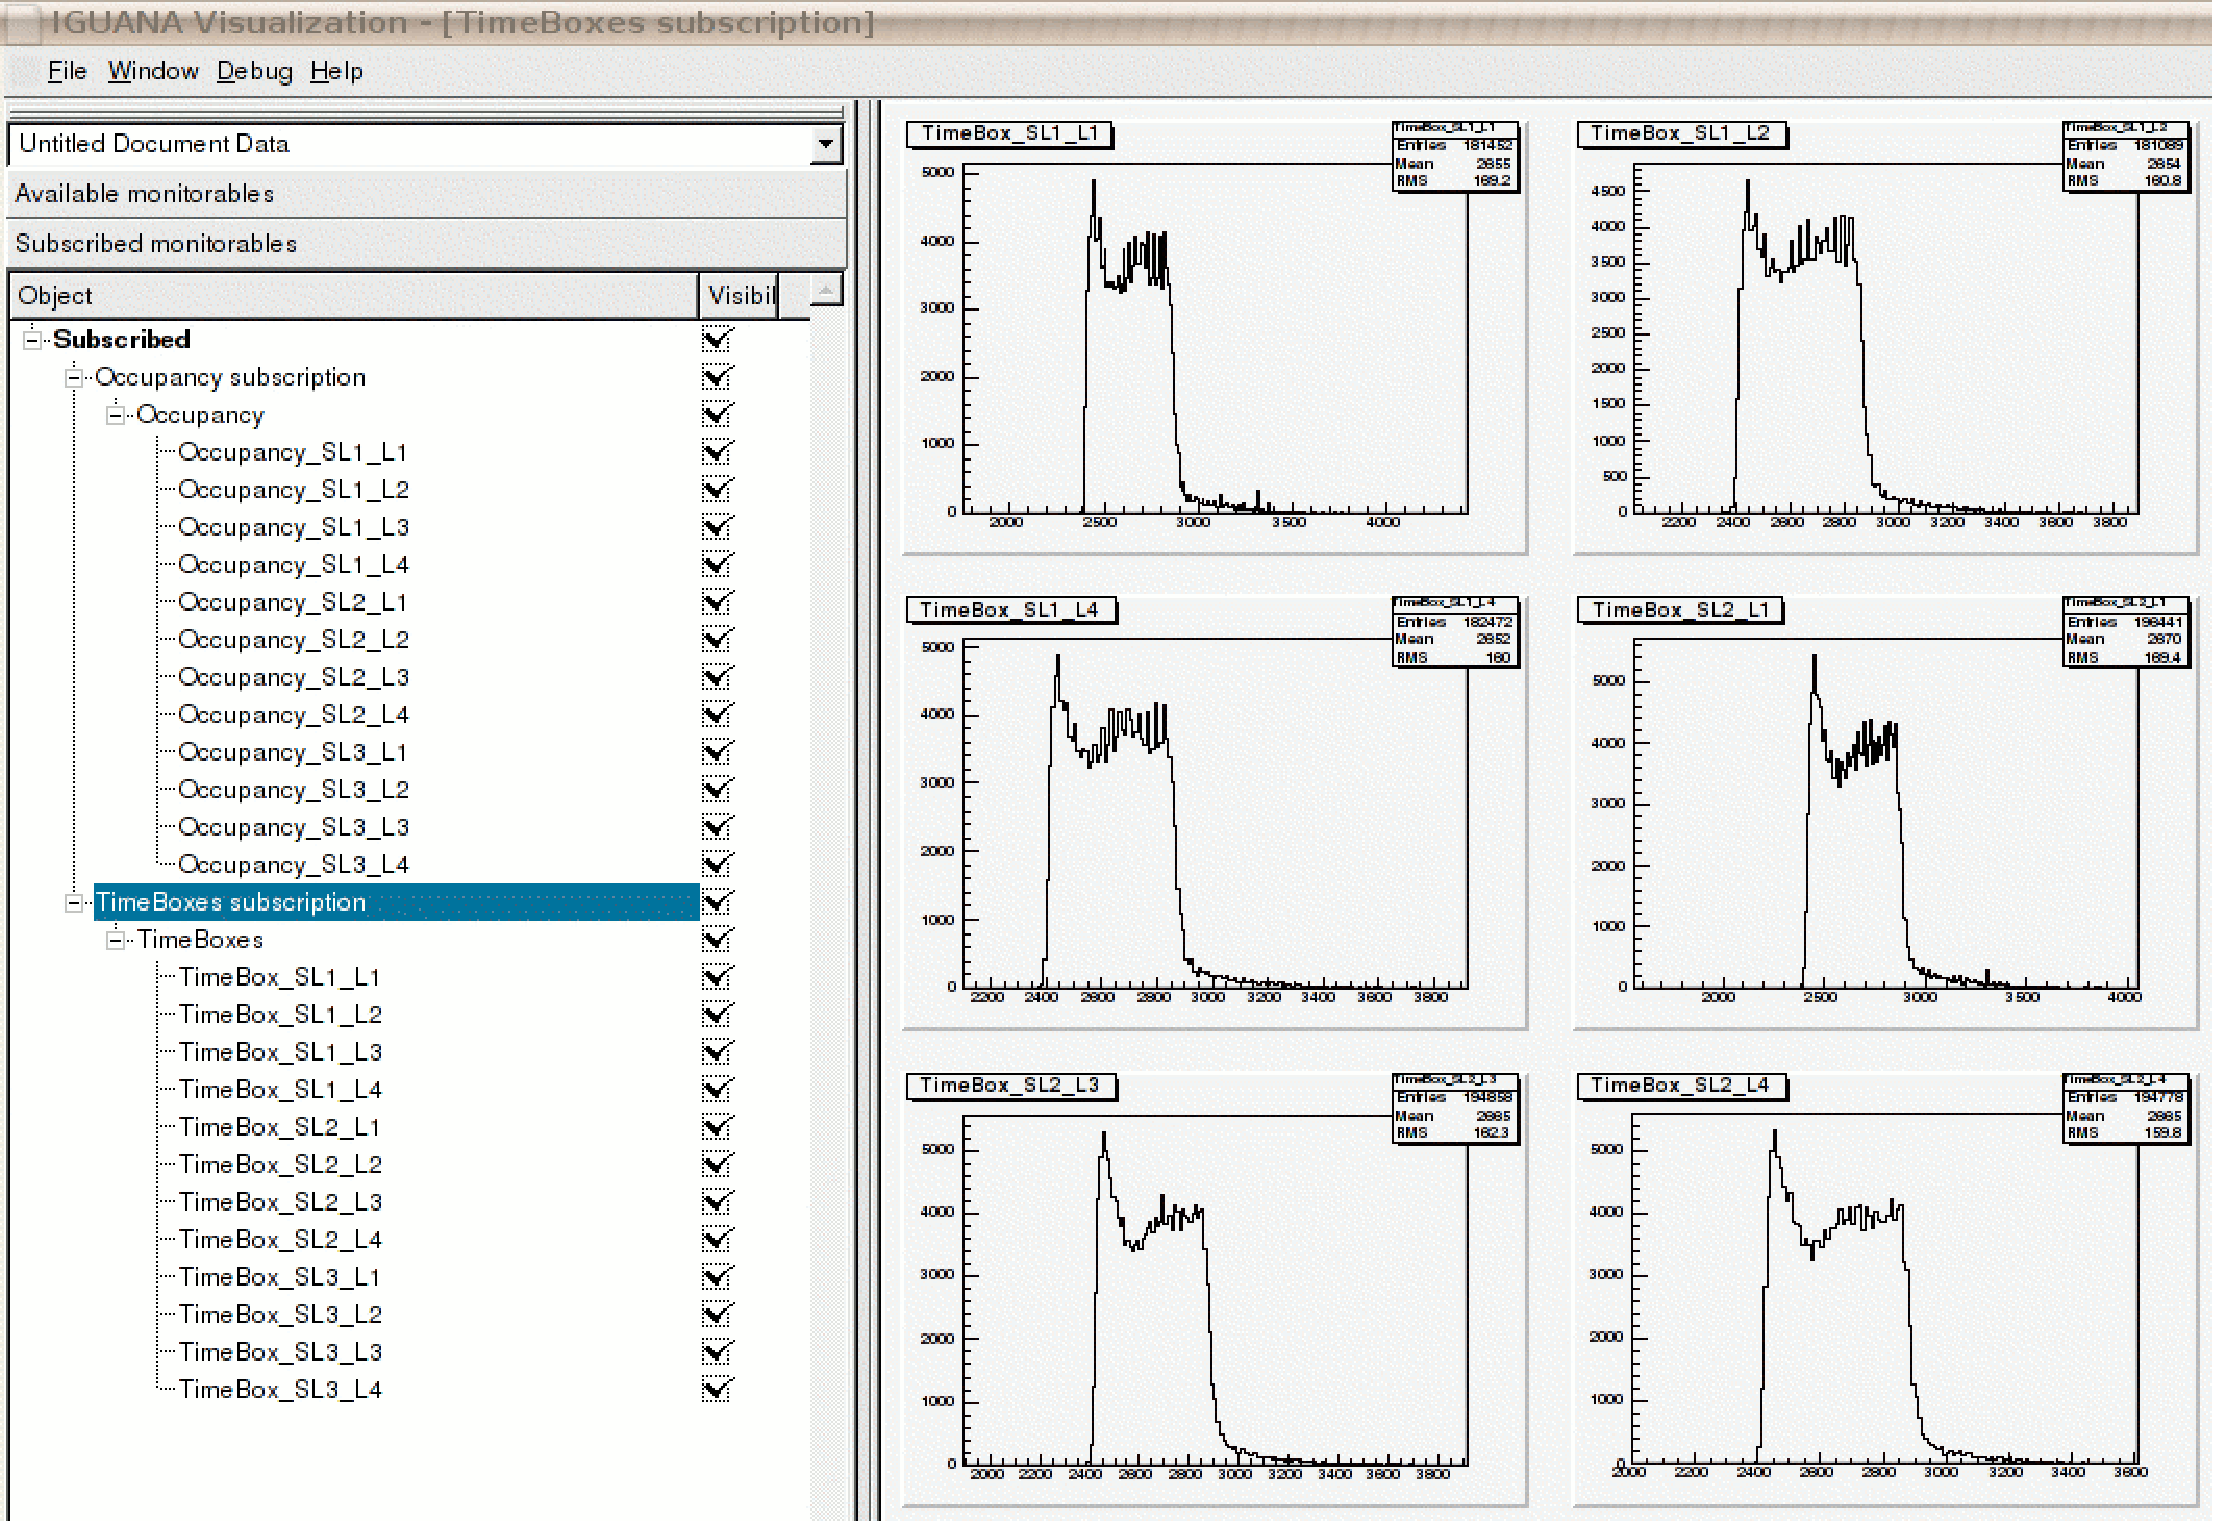
\includegraphics[width=0.9\textwidth]{iguana-dqm}
\caption{Screen shot of the Drift Tubes DQM browser of online data
sources: occupancy and time boxes subscription,
            using the interactive IGUANA  GUI and tree controller to display
            several embedded ROOT canvas components. The data sources are the cosmics muons taken at SX5
during commissioning of the installed DT.\label{iguana-dqm}}
\end{center}
\end{figure}


\section{DQM Commissioning at the Magnet Test and Cosmic Challenge} \label{sec:dqmcommissioning}

While the CMS detector is under construction in the LHC interaction point 5 surface hall, a comprehensive 
programme for commissioning and mapping the coil and operating all subsystems with central trigger and global 
data acquisition has been carried out during fall 2006. These operations are called Magnet Test and Cosmic 
Challenge (MTCC)[MTCC reference]. After having been tested during the preparation for MTCC by individual 
subdetector groups, the DQM has been commissioned and used during the MTCC in a more global setup,
both on-line and quasi on-line in the MTCC control room, and off-line at the Remote Operation Centre at Tier0 (CERN). 


\subsection{Offline DQM at MTCC} \label{sec:dqmcommissioningoffline}
The scope of the offline installation was to create DQM snapshots (in form of root files containing all the available MonitorElement's)
to be stored permanently. The snapshots were created by a DQM Producer which included all the available DQM 
modules relevant to the sub-detectors participating in the final phase of MTCC, i.e. the DQM for HCAL, CSC, DT, RPC, 
for the central trigger board (CTC), a generic module for monitoring the data size of all 
FEDs, and a module for monitoring Muon reconstruction. For all detectors involved the relevant raw data
unpacking code was included. The DQM Producer was the only DQM component run for the off-line application and it was
run in an automated way on all the MTCC data stored in CASTOR[castor reference]. In order to allow users at all CMS sites to view the
snapshots contents through a web browser, a designated AFS area at CERN was used for storage. Fig.~\ref{fig:web_browser_plot} shows an example of
visualizing the DQM snapshots with a web browser.
%
\begin{figure}[hbtp]
  \begin{center}
  \rotatebox{0}{
    \resizebox{12cm}{!}
      {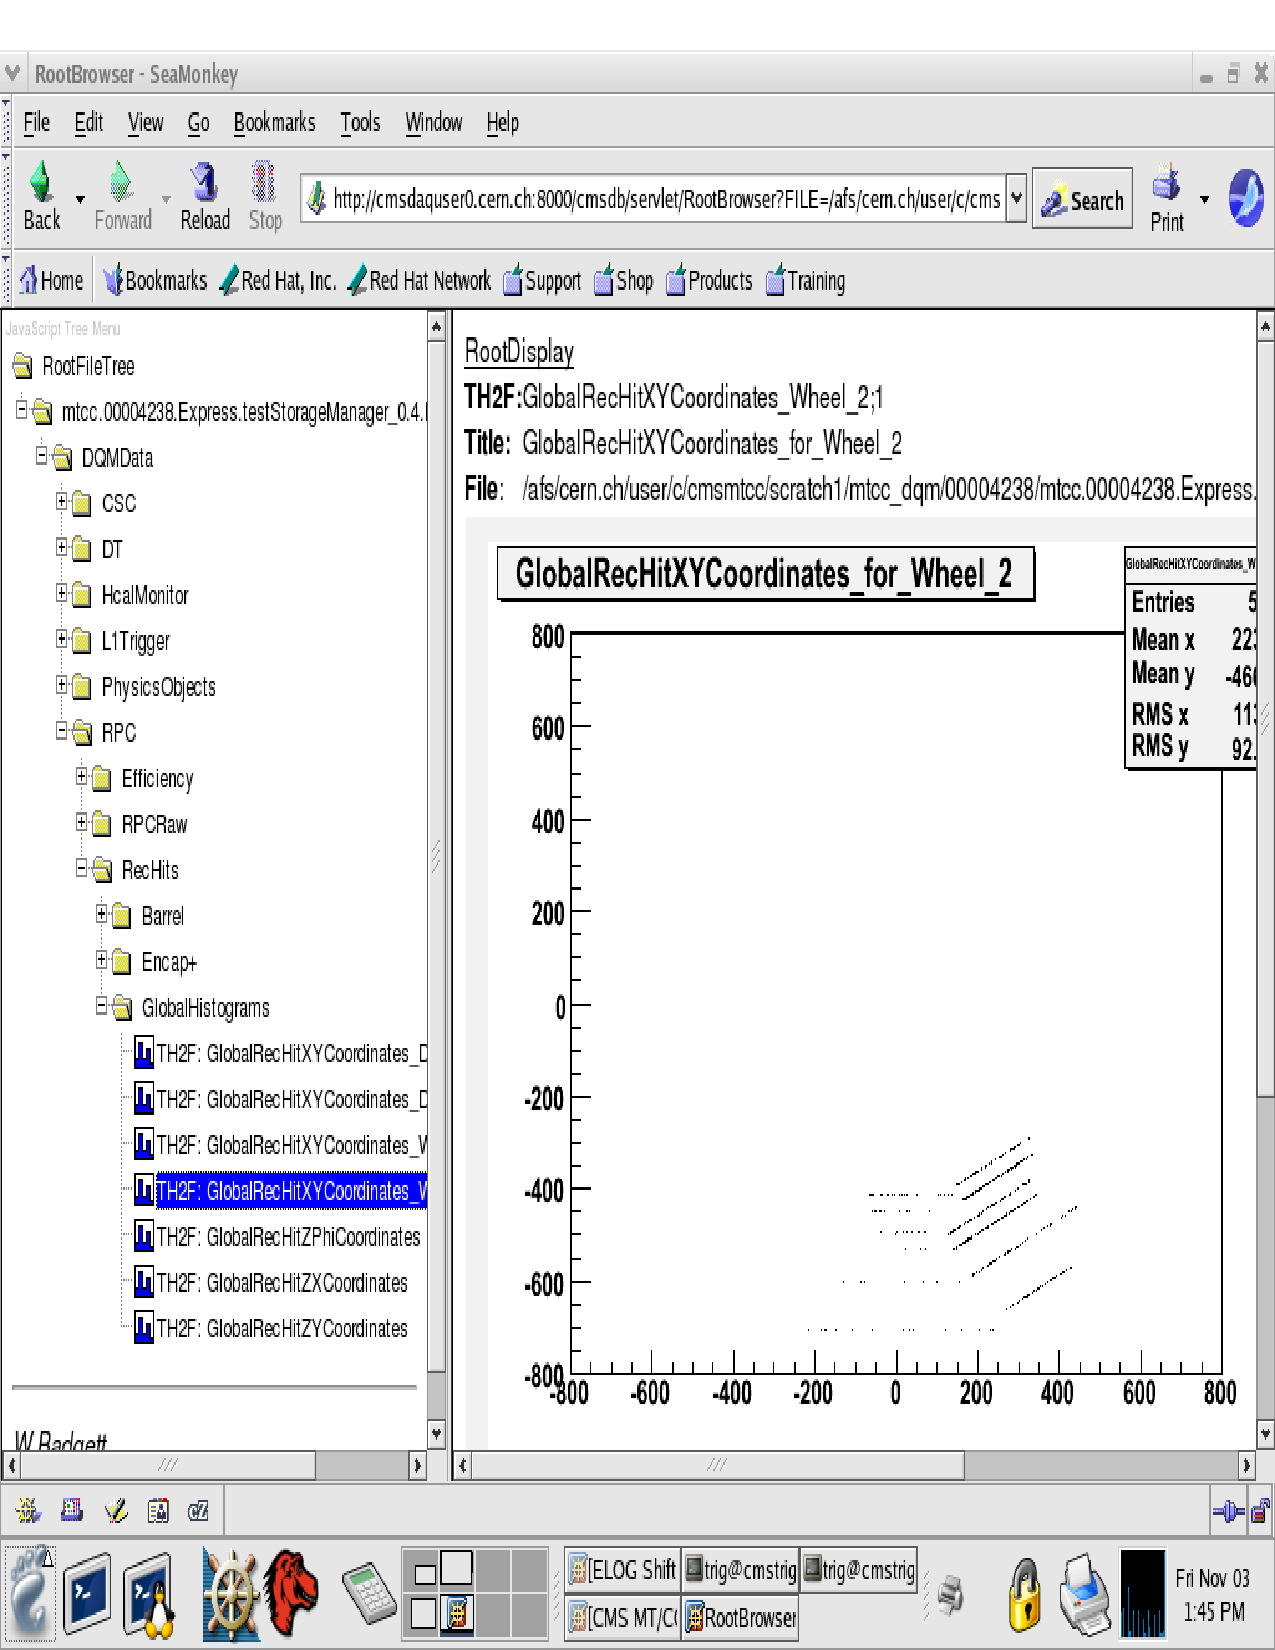
\includegraphics{figures/RPCOfflineIllumination}} 
      }
\caption{DQM snapshots produced off-line at the CERN ROC and visualized with a web browser. The example shows the RPC Chamber illumination plot. On
the left it is visible the directory structure of the root file which can be browsed to select the MonitorElement to view.}
\label{fig:web_browser_plot}
 \end{center}
\end{figure}
%%
%
\begin{figure}[hbtp]
  \begin{center}
  \rotatebox{0}{
    \resizebox{12cm}{!}
      {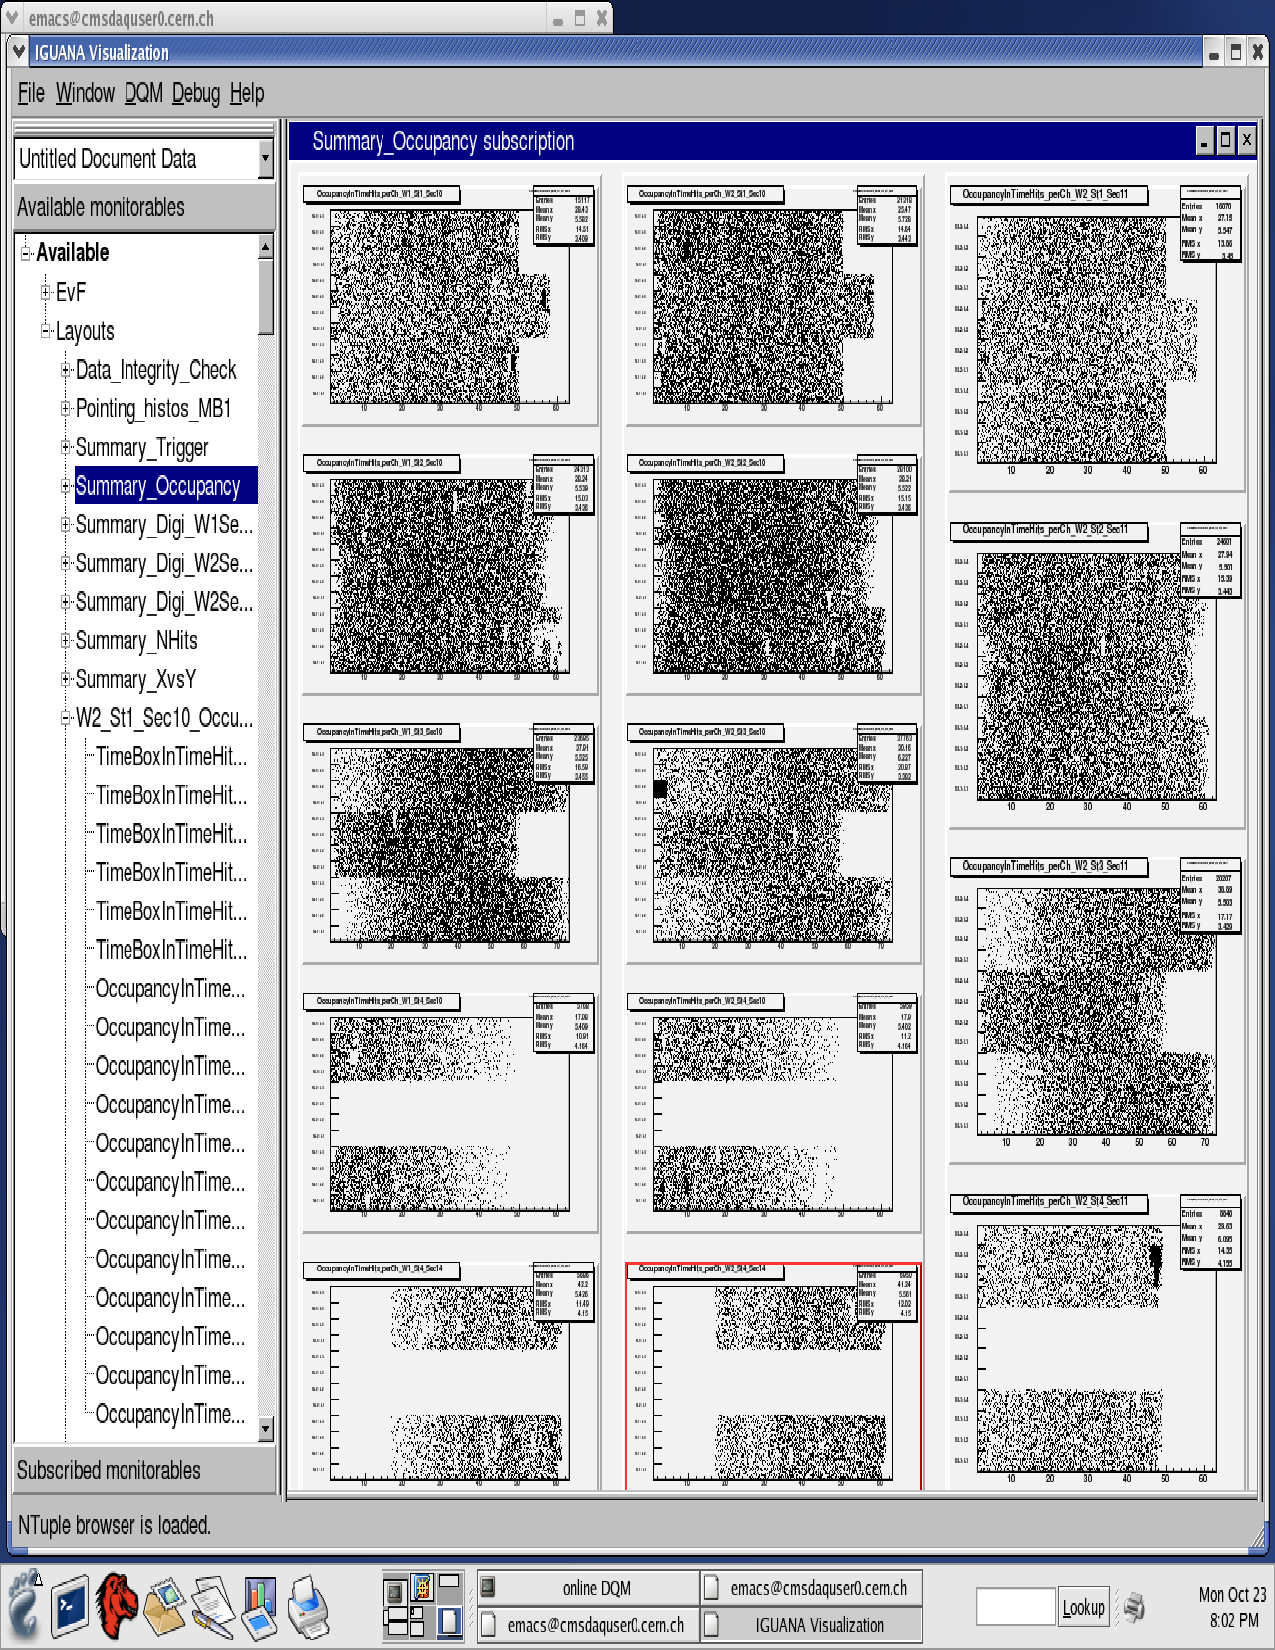
\includegraphics{figures/DTSummaryOccupancy}} }
\caption{DT Integrity check plots (occupancy in time intervals) produced on-line in the Filter Farm and visualized with the Iguana GUI Client.}
\label{fig:dtlayout}
 \end{center}
\end{figure}
%%


\subsection{Online and quasi online DQM at MTCC}

The DQM was used and commissioned in the MTCC control room in an on-line and a quasi on-line setup.
The on-line application included a Producer running in the Filter Farm and one Collector running within the local area network. 
The Producer included the modules for DT, CTC and generic FED monitoring. Clients would be run independently by the groups interested 
in monitoring the data. Fig.~\ref{fig:dtlayout} shows an example of a DT data integrity check MonitorElement collection 
produced in the Filter Farm and visualized with the Iguana GUI by the DT group.

A centralized effort was established for monitoring the data with a quasi-online application. This included a general Producer 
(identical to the one run in the off-line mode, described in subsection~\ref{sec:dqmcommissioningoffline}) consuming events in a 
parasitic way from the StorageManager in parallel to the Event Display[ED reference]. 
For the final two weeks of the MTCC, the Producer was launched by a Run Control Function Manager at the beginning of each run.
One Collector run at all times on a machine visible both
from the control room LAN and from the outside network, this allowed to include some monitoring shifts run from the Remote Operation Centre 
at Fermilab (with the Client run locally at the ROC) in addition to the regular local shifts. 
For these centralized shifts the Iguana GUI Client was used to visualize plots by the users. 
A standard configuration for the monitorable layouts 
was established to accommodate the sub-detector needs and the general interest in visualizing muon reconstruction distributions.
The MonitorElement layouts to be visualized by the shifter included monitorables for DT and RPC data integrity and detector 
functioning checks (with configurations provided by the sub-detector groups), CTC, generic FED's and Muon Reconstruction plots 
(with configurations established within the DQM group). Figure~\ref{fig:muonrecolayout} shows an example of Muon Reconstruction MonitorElements
visualized in the quasi online application.

%
\begin{figure}[hbtp]
  \begin{center}
  \rotatebox{0}{
    \resizebox{12cm}{!}
      {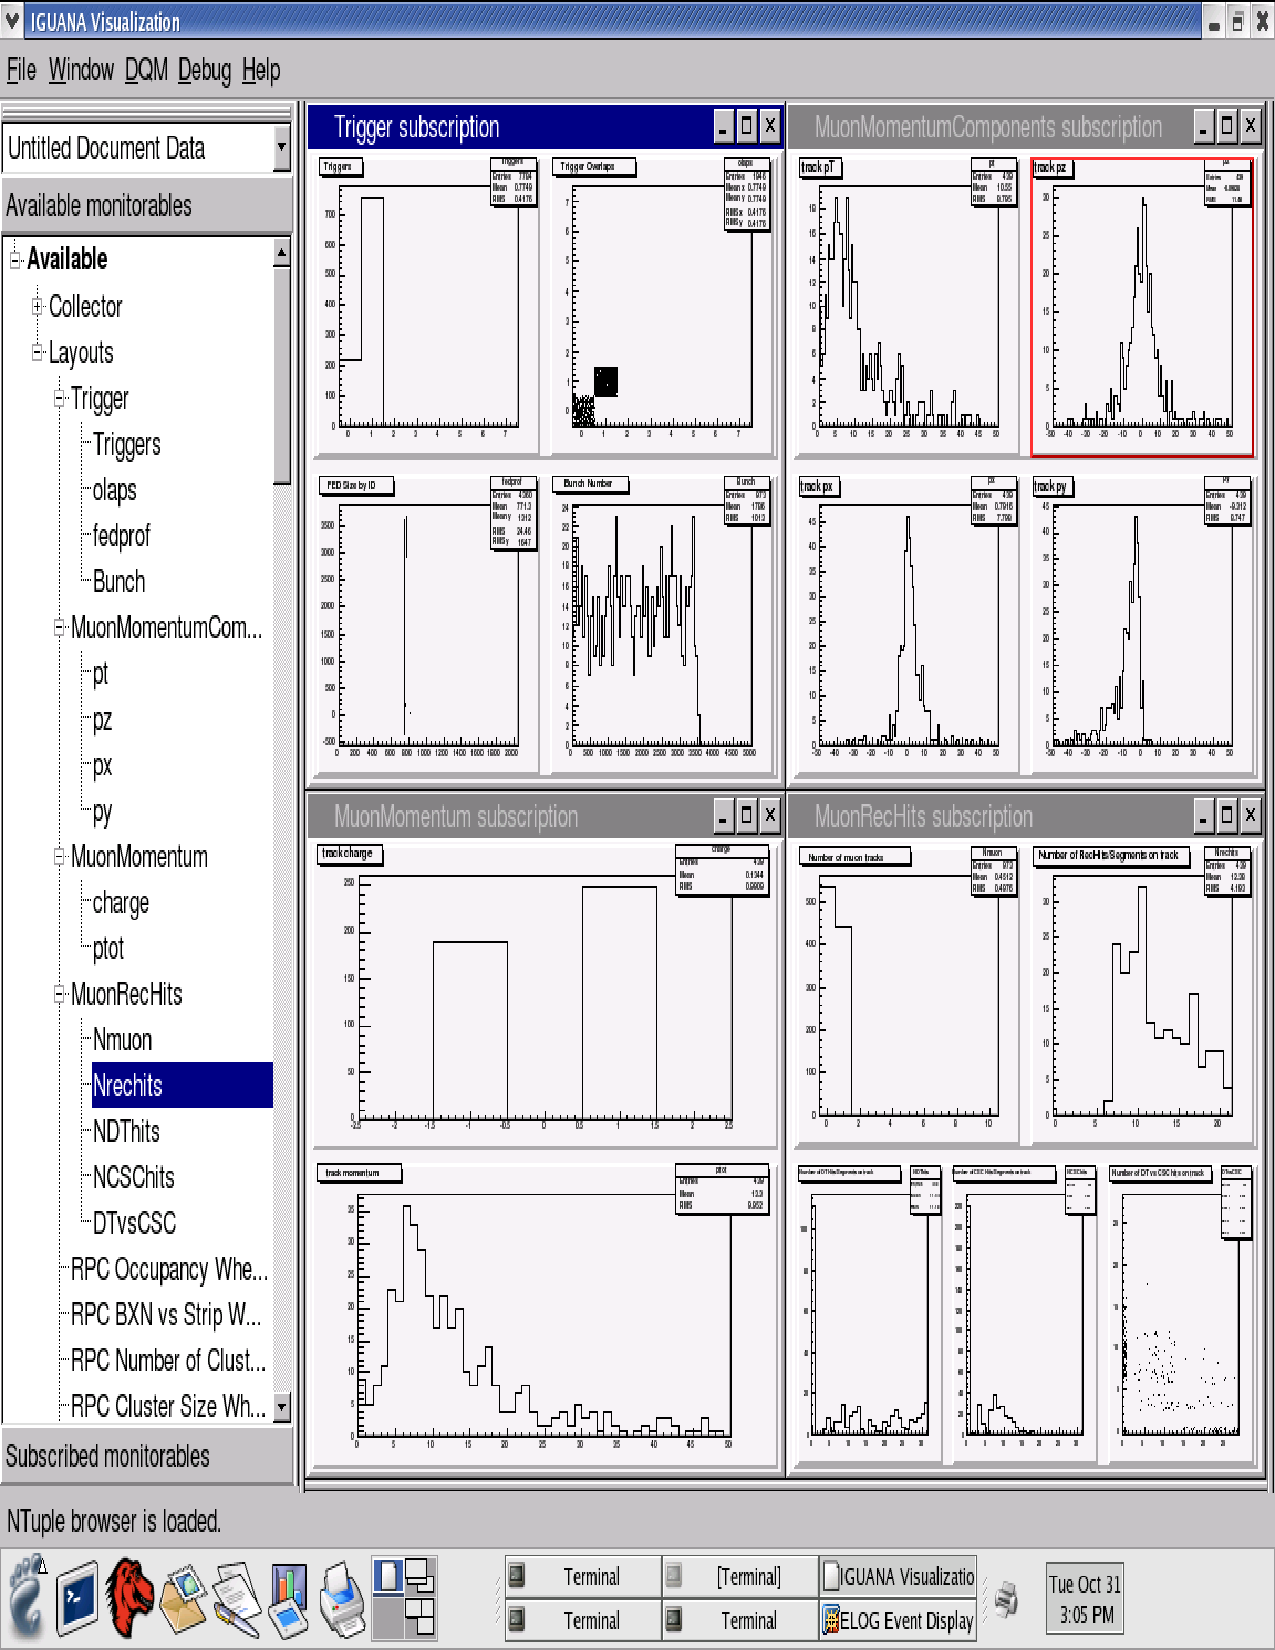
\includegraphics{figures/MuonReco_run4406}} }
\caption{Trigger, FED and Muon Reconstruction MonitorElements produced quasi-online consuming events from Storage Manager and visualized 
with IGUANA GUI. 
The four upper left plots show the Trigger bits distribution, the trigger overlaps, FED size profile and bunch crossing number; 
the four upper right plots show the reconstructed Muon momentum components; 
the two lower left plots show the reconstructed Muon charge and total Momentum; 
the five lower right plots show the number of muons per event reconstructed after level one trigger, the overall (DT and CSC) number 
of hits used in the reconstruction, the number of DT hits used, the number of CSC hits used and the number of DT versus the number of CSC 
hits used.}
\label{fig:muonrecolayout}
 \end{center}
\end{figure}
%%


\subsection{Conclusions on operations}


The DQM was commissioned and used during the fall 2006 CMS Magnet Test and Cosmic Challenge. The main objectives set for DQM in MTCC were met:
a global DQM application was established both for quasi-online and offline operations, DQM (combined with Event Display) shifts were run,
DQM snapshots were saved in permanent storage and some DQM modules were included in the Filter Farm for on-line monitoring. While the overall 
DQM functioning was satisfactory, valuable feedback was achieved from this experience on selected issues that will be addressed. 
In particular, the need of optimizing the efficiency of the individual DQM production modules emerged.
Once shifts for individual sub-detectors will be established in future commissioning programmes and at the LHC startup, 
the inclusion of detector specific information in the centralized shift might become somewhat redundant. 
The centralized DQM installation could then be used for monitoring higher level physical quantities besides the Muon reconstruction
distributions, as for instance  missing energy and invariant masses.



\section{Acknowledgments}

We would like to thank the ROC centre at Fermilab for the remote shifts, the wealth of feedback provided and the web
browsing tools for the DQM snapshots; Martijn Mulders and Frederic Ronga for including the off-line DQM application 
in the automated analysis of the MTCC data; Ianna Osborne for helping in the coordination of the combined DQM and Event Display shifts.


%
%
%================
% Appendix
%================
\newpage
\appendix 
\bigskip

\section{Rationale for accessing monitoring elements via a neutral interface}
%\pdfbookmark[1]{Appendix}{Appendix}
% that does not depend on a specific implementation:
\label{app:neutral_interface}
The current implementation of the monitoring transfer mechanism from a node to
another involves {\tt ROOT} (classes {\tt TSockets}, {\tt
TServerSocket} and {\tt TMessages}). This is out of convenience, since
users have expressed the desire to be able to save monitoring
structures in root-tuples that they can access later. Since the
``behind-the-scenes'' mechanics is implemented with {\tt ROOT}, one 
would be tempted to allow users to deal directly with {\tt ROOT}
objects. However, we have made the choice to hide the ``true'' format
behind a transparent interface for both sources and clients, for a
variety of reasons:
\begin{itemize}
\item{An abstract interface does not bind the user access methods to a
specific analysis framework and/or implementation. In our particular
case, the transfer mechanism and the ``true''
ME format ({\tt ROOT}) could change in the future, without
breaking the source and client programs.}
\item{Having an abstract interface that hides the raw monitoring data from
the user is a good OO practice. The set of allowed operations on the
monitoring objects should be defined by the (abstract) user interface,
not the framework used for the implementation.}
\item{Additional functionality can be added to the monitoring objects
(\eg alarms) without directly inheriting from {\tt ROOT} classes.}
\end{itemize}


\end{document}
